
\documentclass{report}
\usepackage[T1]{fontenc} % Fontes T1
\usepackage[utf8]{inputenc} % Input UTF8
\usepackage[nottoc]{tocbibind}
\usepackage{csquotes}
\usepackage[portuguese]{babel} %Usar língua portuguesa
\usepackage{blindtext} % Gerar texto automaticamentez	
\usepackage[printonlyused]{acronym}
\usepackage{hyperref} % para autoref
%\usepackage[backend=biber, style=ieee]{biblatex}%
\usepackage{graphicx}



\begin{document}
%%
% Definições
%

\def\titulo{Trabalho de aprofundamento AP2}
\def\data{9 de Abril de 2019}
\def\autores{André Patacas, Gil Teixeira}
\def\autorescontactos{(93357) andrepatacas@ua.pt, (88194) gilteixeira@ua.pt}
\def\departamento{Universidade de Aveiro, DETI}
\def\logotipo{ua.pdf}
%
%%%%%% CAPA %%%%%%
%
\begin{titlepage}

\begin{center}
%
\vspace*{50mm}
%
{\Huge \titulo}\\ 
%
\vspace{10mm}
%
{\LARGE \autores}\\ 
%
\vspace{30mm}
%
\begin{figure}[h]
\center
\includegraphics{\logotipo}
\end{figure}
%
\vspace{30mm}
\end{center}
%
\begin{flushright}

\end{flushright}
\end{titlepage}

%%  Página de Título %%
\title{%
{\Huge\textbf{Aplicação para o cálculo de Largura de Banda e de Latência}}\\
{\Large \departamento}
}
%
\author{%
    \autores \\
    \autorescontactos 
}

%
\date{\data}
%
\maketitle

\pagenumbering{roman}






\tableofcontents
\listoftables 
\listoffigures  

%%%%%%%%%%%%%%%%%%%%%%%%%%%%%%%
\clearpage
\pagenumbering{arabic}

%%%%%%%%%%%%%%%%%%%%%%%%%%%%%%%%
%%%%%% RESUMO %%%%%%
\begin{abstract}
Este relatório pretende descrever uma aplicação desenvolvida para calcular a largura de banda e a latência da máquina onde a aplicação se encontra a correr. Calculam-se estes valores para um determinado servidor ou para um conjunto, de cardinalidade especificável, de servidores de um país também este especificável. No final a aplicação cria um relatõrio, (\textit{report.csv}) , em csv, e assina-o com uma chave privada, (\textit{key.priv}), a ser fornecida pelo utilizador.
\end{abstract}

\renewcommand{\abstractname}{Contribuições dos autores}
\begin{abstract}
\textbf{André Patacas}: 50\%
\begin{itemize}
\item Responsável pela elaboração do código da aplicação e pelos testes manuais da aplicação.
\end{itemize}
\textbf{Gil Teixeira}: 50\%
\begin{itemize}
\item Responsável pela elaboração do relatório e pelos testes manuais da aplicação.
\end{itemize}
\end{abstract}

\chapter{Introdução}
\label{chap.introducao}

A aplicação foi desenvolvida em python3 no âmbito da disciplina de Laboratórios de Informática, no ano letivo 2018/2019. A adicionar às especificações básicas pedidas, segundo o guião sobre regras do segundo trabalho de aprofundamento, construiu-se ainda suporte para pydocs, para haja uma explicação mais detalhada de cada classe e método do nosso projeto. O programa foi escrito com base em test driven development  (\autoref{chap.metodologia}) e, como tal, elabourou-se um esqueleto do programa que se pretendia, seguidos pelos testes unitários e finalmente, por vários updates a ambos até chegar ao estado em que a aplicação se encontra. Finalmente é demonstrado em detalhe um exemplo de utilização da aplicação (\autoref{chap:resultados}) e é feita uma conlusão \autoref{chap.conclusao}.


\chapter{Metodologia}
\label{chap.metodologia}

\begin{enumerate}
	\item Criar o esqueleto da aplicação;\\
	Biliotecas usadas:
	\begin{itemize}
	\item \cite[\textit{Documentação sobre a classe socket em C}]{socketsc}
	\item \cite[\textit{Documentação sobre a classe csv em Python 3}]{csvpython}
	\item \cite[\textit{Documentação sobre a classe socket em Python 3}]{socketspython}
	\item \cite[\textit{Documentação sobre a classe pycripto em Python3}]{pycripto}
	\item \cite[\textit{Documentação sobre a classe JSON em Python 3}]{jsonpython}
	\item \cite[\textit{Documentação sobre a classe time em Python 3}]{timepython}
	\end{itemize}
	\item Testar o programa manualmente e com testes unitários;
	\item Criar o primeiro teste (\textit{test\_client}) de forma a que, a cada método que é construido, se possa testar imediatamente se esse método cumpre exatamente com o que estava especificado;
	\item Criar o pydoc para a aplicação e para os testes;
	\item Ajustar os métodos de forma a que a que passem a todos testes;
	\item Iterar o processo de debugging e correção de erros. (\cite[\textit{Stack Overflow}]{stackoverflow})
\end{enumerate}


\chapter{Aplicação de Speed Test}
\label{chap.Aplicação de Speed Test}
\section{client.py}
\label{sec.client}
A forma de utilizar este programa está descrita em detalhe na \autoref{subsec.usage}. Toda a descrição feita neste relatório remete na mesma para a documentação criada a quando do desenvolvimento da aplicação, em pydoc.

\subsection{main}
Ao correr a aplicação a ordem pela qual os métodos são chamados é a seguinte:
\begin{enumerate}
\item \nameref{subsec:loadserver} - \autoref{subsec:loadserver};
\item \nameref{subsec.validate} - \autoref{subsec.validate};
\item \nameref{subsec.runt} - \autoref{subsec.runt};
\item \nameref{subsec.report} - \autoref{subsec.report};
\item \nameref{subsec.signDoc} - \autoref{subsec.signDoc}.
\end{enumerate}

\subsection{usage()}
\label{subsec.usage}
Este método imprime a mensagem de erro passada como argumento e imprime a ajuda para utilização da aplicação. No campo \textit{option} pode usar \textit{-v} para entrar em modo verbose.\\ 
\textbf{Argumentos}: \textit{message} (str).\\
\textbf{Retorna}: \textit{None}.

\subsection{validate()}
\label{subsec.validate}
Este método trata da validação dos argumentos passados pela variávle sys.argv.\\ 
\textbf{Argumentos}: \textit{None}.\\
\textbf{Retorna}: \textit{None}.

\subsection{run\_tests()}
\label{subsec.runt}
Este método serve para calcular a largura de banda e latência da conexão a um \textit{num} de servidores num país, ou a um server com o id passado por argumento.\\
Nota: se o terceiro argumento for um id, a função realizará \textit{num} testes a esses servidor, se for um país, fará \textit{num} testes usando a função \autoref{subsec.countrytest} e se não foi passado terceiro argumento realiza um teste random (\autoref{subsec.randt}).\\
\textbf{Argumentos}: 
\begin{enumerate}
\item \textit{inteval}: intervalo de tempo entre cada teste realizado;
\item \textit{num}: número de testes a realizar;
\item \textit{id\_or\_country}: país (str) ou id (int) de um server;
\item \textit{option}: -v se pretender correr a aplicação em modo \textit{verbose}.
\end{enumerate}
\textbf{Retorna}: objeto \textit{SpeedTestResult} com as informações relativas aos resultados do teste.

\subsection{country\_test()}
\label{subsec.countrytest}
Este método serve para calcular a largura de banda e latência da conexão a um servidor aleatório do país passado como argumento.\\ 
\textbf{Argumentos}: (str) \textit{target\_country}.\\
\textbf{Retorna}: objeto \textit{SpeedTestResult} com as informações relativas aos resultados do teste.

\subsection{id\_test()}
\label{subsec.idtest}
Este método serve para calcular a largura de banda e latência da conexão a um servidor com o id passado como argumento.\\ 
\textbf{Argumentos}: (int) \textit{target\_id}.\\
\textbf{Retorna}: objeto \textit{SpeedTestResult} com as informações relativas aos resultados do teste.

\subsection{random\_test()}
\label{subsec.randt}
Este método serve para calcular a largura de banda e latência da conexão a um servidor random.\\ 
\textbf{Argumentos}: \textit{None}.\\
\textbf{Retorna}: objeto \textit{SpeedTestResult} com as informações relativas aos resultados do teste.


\subsection{calc\_download()}
\label{subsec.download}
Cálculo de largura de banda.\\
Este método pede ao \textit{target\_server} um download de 100 mb. Durante 10 segundos é feito download dos dados enviados pelo mesmo. No final dos 10 segundos, se o download tiver sido superior a 10mb regista, caso contrário, discarta este servidor.\\
\textbf{Argumentos}: \textit{target\_server}(dicionário com informação sobre o target server). 
\textbf{Retorna}: (float) $\textit{len(buffer)}/\textit{(e\_time * MB)}$

\subsection{calc\_latency()}
\label{subsec.latency}
Cálculo da latência.\\ 
Este método troca dez \textit{PING-PONG} com o \textit{target\_server} e calcula o tempo médio em milisegundos entre estas trocas.\\
\textbf{Argumentos}: target server (dicionário com informação sobre o target server). 
\textbf{Retorna}:(int) \textit{average\_trade\_time} em ms.

\subsection{report()}
\label{subsec.report}
Este método vai gerar um \textit{test\_report} baseado numa lista de objetos \textit{SpeedTestResult} passados como argumentos.\\ 
\textbf{Argumentos}:
\begin{enumerate}
\item List[objeto \textit{SpeedTestResult}];
\item \textit{report\_name} (str) - nome do ficheiro a ser gerado.
\end{enumerate}
\textbf{Retorna}: \textit{None}. O ficheiro \textit{test\_report} será gerado

\subsection{create\_signed\_document}
\label{subsec.signDoc}
Este método gera um \textit{signature file} assinando o \textit{report} com a chave privada no \textit{key\_path} especificada. A chave tem 128 bits e o texto é assinado de 16 em 16 caracteres, por isso deve ser verificado da mesma forma (ver \autoref{subsec.signDoc}). \\ 
\textbf{Argumentos}: 
\begin{enumerate}
\item \textit{key\_path} (str): O \textit{path} para a localização da chave;
\item \textit{report\_name} (str): Nome do \textit{report} a ser assinado;
\item \textit{signature\_name} (str): Nome do \textit{signature file} que será gerado.	
\end{enumerate}
\textbf{Retorna}: \textit{None}.

\subsection{log()}
\label{subsec:log}
Este método imprime a mensagem passada como argumento, com a cor passada como argumento.\\ 
\textbf{Argumentos}: 
\begin{enumerate}
\item \textit{message} (str);
\item \textit{colour} (str).
\end{enumerate}
\textbf{Retorna}: \textit{None}.

\subsection{log\_error()}
Este método chama \autoref{subsec:log} com a mensagem igual à passada como argumento mas com cor vermelho.\\ 
\textbf{Argumentos}:
\textit{message} (str).\\
\textbf{Retorna}: \textit{None}.

\subsection{log\_warning()}
Este método chama \autoref{subsec:log} com a mensagem igual à passada como argumento mas com cor amarela.\\ 
\textbf{Argumentos}:
\textit{message} (str).\\
\textbf{Retorna}: \textit{None}.

\subsection{log\_verbose()}
Este método chama \autoref{subsec:log} com a mensagem igual à passada como argumento mas com cor verde se o modo \textit{verbose} estiver ativado.\\ 
\textbf{Argumentos}:
\textit{message} (str).\\
\textbf{Retorna}: \textit{None}.

\subsection{load\_server()}
\label{subsec:loadserver}
Este método lê o ficheiro \textit{"servers.json"} e cria um dicionário global com a lista de servidores.\\
\textbf{Argumentos}:
\textit{None}.\\
\textbf{Retorna}: \textit{None}.

\section{test\_client}
Este programa é constituida por métodos que são testes unitários aos da aplicação principal (\autoref{sec.client}). Lista de funções com testes unitários:
\begin{enumerate}
\item test\_calc\_download() : \autoref{subsec.download};
\item test\_calc\_latency(): \autoref{subsec.latency};
\item test\_country\_test(): \autoref{subsec.countrytest};
\item test\_create\_signed\_document(): \autoref{subsec.signDoc};
\item test\_id\_test(): \autoref{subsec.idtest};
\item test\_random\_test(): \autoref{subsec.randt};
\item test\_report(): \autoref{subsec.report};
\item test\_run\_test(): \autoref{subsec.runt}.
\end{enumerate}

\section{speed\_test\_result}
Este programa serve para criar objetos SpeedTestResult que têm, cada um, as informações respetivas a um teste. Tem apenas um construtor e um método:
\subsection{Construtor}
O construtor da classe cria um objeto com os parametros passados como argumentos:
\textbf{Argumentos}:
\begin{enumerate}
\item \textit{server\_id} (int);
\item \textit{download\_speed} (float);
\item \textit{latency} (int);
\end{enumerate}

\subsection{getObjDict}
Este método devolve um dicionário com os resultados do teste relativo ao objeto. O último elemento do dicionário é o resultado do processo de hashing por SHA256 dos atributos anteriores concatenados.\\
\textbf{Argumentos}: \textit{None}.\\
\textbf{Retorna}: \textit{testResult} (dict).
\chapter{Resultado}
\label{chap:resultados}
\section{Exemplo de utilização 1}
\label{sec:example1}
Com exemplo ir-se-á correr a aplicação \autoref{sec.client} com os argumentos:
\begin{enumerate}
\item \textit{interval} = 5 (segundo);
\item \textit{num} = 3 (testes);
\item \textit{id\_or\_country} = Portugal;
\item \textit{option} = -v (\textit{verbose}).
\end{enumerate}

Ao correr a aplicação com estes argumentos, segundo a \autoref{subsec.usage}, vêm os seguintes resultados:
\begin{figure}[h]
	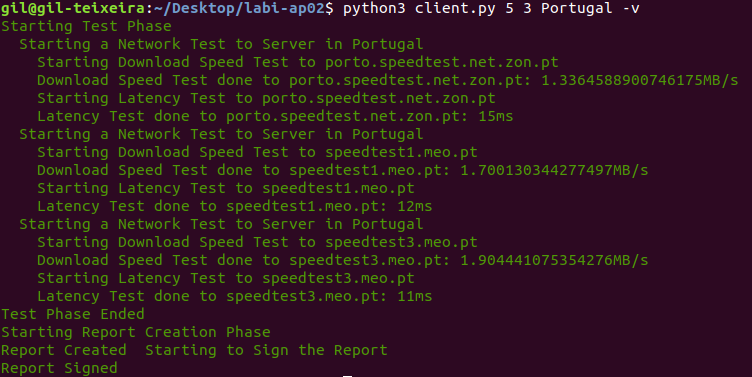
\includegraphics[width=\textwidth]{useExample1}
	\caption{Figura 1}
\end{figure}
\\Criando-se dois novos ficheiros na pasta onde está a aplicação:
\begin{itemize}
\item report.sig, contendo uma assinatura do relatório pela chave privada fornecida (\textit{key.priv}).
\item report.csv, um ficheiro \ac{csv} com os resultados dos três testes efetuados:
\end{itemize}
\begin{table}[h]
\caption{Tabela 1}
\centering
\resizebox{\textwidth}{!}{%
\begin{tabular}{llllll}
Contador & Id Do Servidor & Data e Hora no Formato ISO & Latencia & Largura de Banda & Check \\
1 & 9729 & 2019-04-19 23:04:48.745678 & 13 & 1.3335593613565648 & aa8c139784e517d2f79a785fa224767b8714d494d8a4ede60a755c184019763e \\
2 & 9729 & 2019-04-19 23:05:03.921081 & 14 & 1.682293124975788 & d12a70a22302919711a5f9233340b27b6cfeb4d2ac81ed2f3575048bca51012a \\
3 & 1902 & 2019-04-19 23:05:19.024825 & 6 & 1.882504664392915 & 2f1b6bc5511c4db3e74143fc903bf11a82dad81d0dcbf6b2fb3927af85542c1e
\end{tabular}%
}
\end{table}

\section{Exemplo de utilização 2}
\label{sec:example2}
Com exemplo ir-se-á correr a aplicação \autoref{sec.client} com os argumentos:

\begin{enumerate}
\item \textit{interval} = 1 (segundo);
\item \textit{num} = 20 (testes);
\end{enumerate}

Ao correr a aplicação com estes argumentos, segundo a \autoref{subsec.usage}, vêm os seguintes resultados:

\begin{figure}[h]
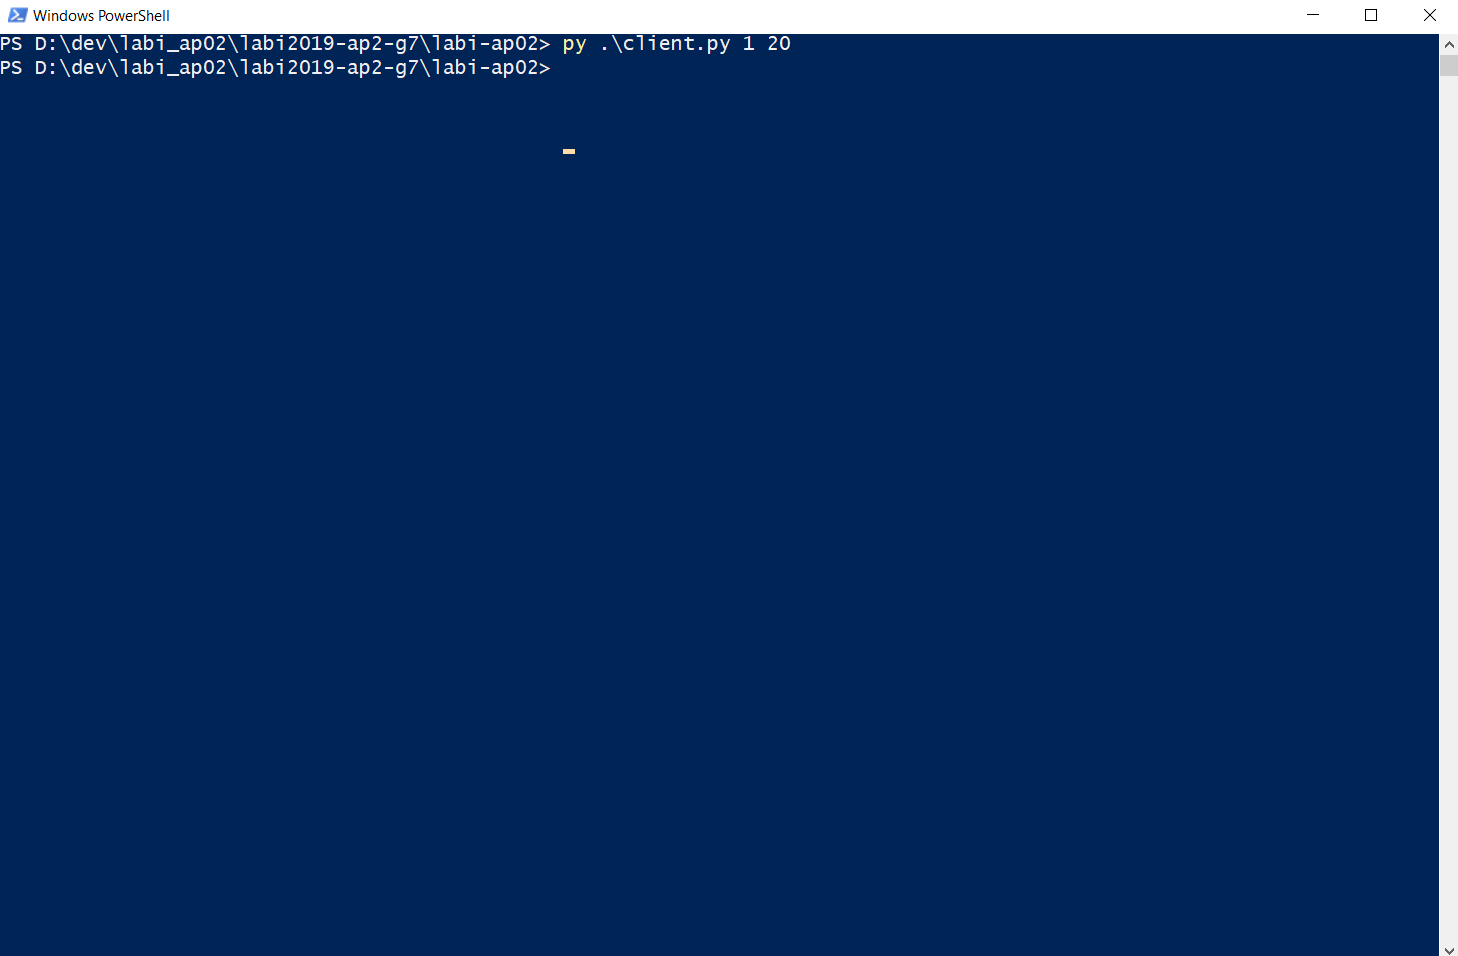
\includegraphics[width=\textwidth]{useExample2}
\caption{Figura 2}
\end{figure}

Criando-se dois novos ficheiros na pasta onde está a aplicação:

\begin{itemize}
\item report.sig, contendo uma assinatura do relatório pela chave privada fornecida (\textit{key.priv}).
\item report.csv, um ficheiro \ac{csv} com os resultados dos vinte testes efetuados:
\end{itemize}

\begin{table}[h]
\caption{Tabela 2}
\centering
\resizebox{\textwidth}{!}{%
\begin{tabular}{llllll}
	Contador & Id Do Servidor & Data e Hora no Formato ISO & Latencia & Largura de Banda   & Check                                                            \\
	1        & 3787           & 2019-04-23 23:15:11.814397 & 72       & 1.2450874408544983 & e3303529e750ab6fbf6e3657bc981911ef7db2f3df67ae11ab6a19d17ac3a1ed \\
	2        & 6907           & 2019-04-23 23:15:25.371232 & 200      & 1.453856874134937  & 0dce75c41407aade02ac0552bcd5f5d3340e6849815cf0a4e4adc1aed55edd0c \\
	3        & 12322          & 2019-04-23 23:15:40.323813 & 301      & 1.6721249958527682 & 602ea564434909e5b1471b22b51d0e8ce6311e2499ac0ecf6e0d51b8bd76aea7 \\
	4        & 13606          & 2019-04-23 23:15:55.476764 & 300      & 0.3002715865565481 & 69e5586b72267a7629471b90506d27bc4e56b86572129603657bcef0c4beceed \\
	5        & 21873          & 2019-04-23 23:16:10.429150 & 305      & 0.6919384792792023 & becdbf5a489547184f0ee5dee68f7a9c7ef3d7766c251b524935b5744aee817b \\
	6        & 20978          & 2019-04-23 23:16:22.785171 & 96       & 1.8346690686226794 & 06727d7d25aba259931278f2d543a5fdad855d8f32c602eace5cea441c6bf4ac \\
	7        & 10728          & 2019-04-23 23:16:38.828644 & 301      & 0.210595319242981  & 58fdd5509cbe10a36352cf9f47f0ff5ca29bf5f67d27732fb847686ee97dcf6b \\
	8        & 3482           & 2019-04-23 23:16:51.987782 & 164      & 1.8180169922073217 & e0e9678472c4405a8a042c29dd20b71e5d8cfb6058dc353aca592f0c9efeb6c5 \\
	9        & 7035           & 2019-04-23 23:17:05.421876 & 188      & 1.9264675928248938 & 37b6d7f555e0e856812fc3f524067dd37d642c4f234d7d3300be9ad296b3a9f7 \\
	10       & 9566           & 2019-04-23 23:17:20.374519 & 298      & 1.8944690340216246 & 0ac63397a48e204307f91ffdd92b95eacb50d7910895f5d7eddc66ba5c544f0c \\
	11       & 3555           & 2019-04-23 23:17:32.722854 & 94       & 2.0166120335557522 & abd80b26ec548bf56caab155544ca524bb516072db9d2cfea28f738354a7f67c \\
	12       & 2845           & 2019-04-23 23:17:47.773268 & 324      & 1.8117547004538457 & f001cd88c662dde20635deae16c37504354ad263ac5b8ce04a08eb595f037d21 \\
	13       & 10230          & 2019-04-23 23:17:59.925717 & 87       & 2.057615821157388  & 88a60195bd227a14ffb815da2d3d622465a86f983f277f1c45f3c28cf9ddf84b \\
	14       & 1609           & 2019-04-23 23:18:13.560844 & 200      & 2.063724927825838  & de7f4db37eb5d6d15c4de242cf585c066c8710c33e46386d224a65602ad2bce9 \\
	15       & 17427          & 2019-04-23 23:18:28.513233 & 299      & 1.1734104673200632 & f39c6fba23407b29e7d4df5ef0391d8d505b9455ae8ccf0c2482324285914c28 \\
	16       & 19534          & 2019-04-23 23:18:42.161013 & 192      & 1.1744314579010149 & 76e3df9180d78aa4f50ebb7d30ccb105364ec910ac3ecf5de84d07e37c25db4f \\
	17       & 10420          & 2019-04-23 23:18:54.102702 & 75       & 2.132581818908019  & 5c563bf487f06307a53d79d28b486b82afdc08d687cf34969e9e7edc61fded5b \\
	18       & 19866          & 2019-04-23 23:19:08.813828 & 300      & 1.974450059487398  & e320d4a4da6fa85634760c6d7e0aa7b786d9c74b4ed5a27fb39dd18a979944ab \\
	19       & 16635          & 2019-04-23 23:19:23.506009 & 305      & 1.8385825253261963 & 027bb4e49c96ca3abe104c74adb30f18a5c3c0a5d8c52c8d6c7a221259e9d1c7 \\
	20       & 1369           & 2019-04-23 23:19:38.659193 & 301      & 0.3467424459681414 & 18b151603cc853562f6041b0c1a59d3acbc5c0eb0260bb86c90fac52ed3ef8f8	
\end{tabular}%
}
\end{table}

\chapter{Conclusão}
\label{chap.conclusao}
Dos testes feitos pode concluir-se que a latência depende diretamente da distância geográfica ao local do \textit{target\_server}, sendo tanto maior quanto maior a distância entre a máquina e o server. Por outro lado parece existir uma inconsistência na relação entre a distância e a velocidade de \textit{download} o que pode indicar que está dependa da qualidade da infraestrutura do país em questão.


\chapter*{Acrónimos}
\begin{acronym}
\acro{ua}[UA]{Universidade de Aveiro}
\acro{miect}[MIECT]{Mestrado Integrado em Engenharia de Computadores e Telemática}
\acro{guiaomini}[Mini-projeto]{Universidade de Aveiro
		Dep. de Electrónica, Telecomunicações e Informática
		Laboratório de Sistemas Digitais}
\acro{csv}[CSV]{Comma Separated Values}
\end{acronym}
%%%%%%%%%%%%%%%%%%%%%%%%%%%%%%%%%







\bibliographystyle{plain}
\bibliography{bibliografia}














%%%%%%%%%%%%%%%%%%%%%%%%%%%%%%%%%


\end{document}
